%%%%%%%%%%%%%%%%%%%%%%%%%%%%%%%%%%%%%%%%%%%%%%%%%%%%%%%%%%%%%%%%%%%%%%%%%%%%%%%
% intro.tex: Introduction to the thesis
%%%%%%%%%%%%%%%%%%%%%%%%%%%%%%%%%%%%%%%%%%%%%%%%%%%%%%%%%%%%%%%%%%%%%%%%%%%%%%%%
\chapter{Introduction}
\label{intro_chapter}

\begin{refsection}
%%%%%%%%%%%%%%%%%%%%%%%%%%%%%%%%%%%%%%%%%%%%%%%%%%%%%%%%%%%%%%%%%%%%%%%%%%%%%%%%

In 1915, Einstein's theory of general relativity (GR) was published, and in it was a revolutionary understanding of the relationship between energy density and the geometry of spacetime~\cite{Einstein:1916vd}.
More than a century later, GR has withstood every test that has been made against it.
One such test of GR was the prediction of gravitational waves (GWs), which are weak perturbations to the spacetime metric that take the form of a wave equation.
Though they represent a straightforward consequence of the equations of GR, it was not until 1974 that GWs were first indirectly detected by the discovery of the Hulse-Taylor binary pulsar system~\cite{HuTa1975} and the subsequent analysis of its decaying period due to emission of GWs~\cite{TaWe1982}.
The first direct measurement of GWs came more than 50 years later, a century after Einstein's publication, when the LIGO detectors~\cite{Aasi_2015} observed the merger of a binary black hole (BBH) system in 2015~\cite{AbEA2016a}.

The LIGO detectors are a pair of ground-based interferometric detectors, located in Hanford, Washington and Livingston, Louisiana.
Since that time, they have been joined by the Virgo~\cite{Acernese_2015} and KAGRA~\cite{kagra} detectors, located in Italy and Japan, respectively.
There are also plans for future ground-based detectors, Cosmic Explorer~\cite{Evans_2021} and Einstein Telescope~\cite{Punturo_2010}, as well as a space-based detector, the Laser Interferometer Space Antenna (LISA)~\cite{LISA2000}.
All of these detectors operate under the same principle, seeking to detect a change in the relative position of test masses as GWs pass through them.

Over the past decade, as instruments have been upgraded and made more sensitive, the catalog of GW detections has grown.
The LIGO-Virgo-KAGRA collaboration (LVK) has reported hundreds of signals from compact binary coalescences (CBCs)~\cite{LIGOScientific:2025slb}, most of which are BBHs, but a few come from neutron star -- black hole (NSBH) mergers, and one has come from a binary neutron star (BNS) merger~\cite{AbEA2017b}.
The observation of the BNS merger was a landmark event for astrophysics because it was observed not only via GWs, but also across the electromagnetic (EM) spectrum~\cite{AbEA2017f}.
The scarcity of such a scientifically interesting phenomenon has motivated much of the work in this dissertation.

In the remainder of Chapter~\ref{intro_chapter}, I will give a brief overview of the mathematics of GR and how GWs appear as a solution to its equations in Sec.~\ref{intro_sec:gr-math}.
In Sec.~\ref{intro_sec:gr-source}, I will discuss sources of GWs with a focus on CBCs.
In Sec.~\ref{intro_sec:detectors}, I will discuss the operation of the LIGO interferometers.
In Sec.~\ref{intro_sec:matched_filter}, I will describe matched filtering, the traditional technique used to search for GW signals in detector data.
In Sec.~\ref{intro_sec:bayesian_pe}, I will introduce Bayesian parameter estimation, the standard framework for measuring source properties from detected GW signals.
Matched filtering and Bayesian parameter estimation provide the baseline against which the ML methods in this dissertation are compared.
Finally, in Sec.~\ref{intro_sec:ml}, I will introduce the machine learning approaches used in this dissertation, motivating the algorithmic choices made in subsequent chapters.

Chapter~\ref{chap:aframe_methods} introduces a machine learning-based method for the detection of gravitational waves from CBCs.
I will outline this method and present a comparison to existing search pipelines used by the LVK.
This algorithm is shown to have similar sensitivity to BBH mergers, while reporting events at much lower latencies.

Chapter~\ref{chap:o3_catalog} presents the results of applying this method to data from LIGO's third observing run, O3. 
Detections are compared to those of other searches, and new candidate events are discussed.

Chapter~\ref{chap:amplfi_methods} introduces a companion machine learning algorithm for the characterization of detected gravitational waves in a low-latency environment.
The algorithm uses normalizing flows to estimate the posterior distributions of parameters of interest (chirp mass, mass ratio, sky location) in under 2 seconds, significantly faster than traditional methods.

Chapter~\ref{chap:amplfi_results} demonstrates this algorithm's performance on mock data from O3.
It is shown to have performance equivalent to existing low-latency methods for signal localization, and to have posteriors consistent with those of the full Bayesian parameter estimation done for the third gravitational wave transient catalog, GWTC-3.

In Chapter~\ref{chap:online}, I discuss how the search and parameter estimation algorithms were combined into a real-time search.
The two were deployed into a production setting at the end of August, 2025, joining the end of the final part of the fourth observing run, O4c.
Public results from that time period are presented.

Finally, in Chapter~\ref{conclusion_chapter}, I highlight ongoing efforts to improve these tools and conclude with a discussion of prospects for the future.

\section{General Relativity and Gravitational Waves}
\label{intro_sec:gr-math}

In this section, I will give a brief description of how the existence of GWs follows from the equations of general relativity.
I will follow the standard ``Einstein notation'', where repeated upper and lower indices imply summation over that index; i.e., $a_\mu b^\mu \equiv \sum_{\mu=0}^3 a_\mu b^\mu$.
In what follows, Greek indices ($\mu$, $\nu$, etc.) run from 0 to 3 and indicate full spacetime coordinates, while Latin indices ($i$, $j$, etc.) run from 1 to 3 and indicate spatial coordinates.

The field equations of GR relate the geometry of spacetime to the density and flux of energy.
These are a set of ten non-linear differential equations, written compactly as:
\begin{equation}
    G_{\mu\nu} = \frac{8\pi G}{c^4} T_{\mu\nu}
\end{equation}
where the Einstein tensor $G_{\mu\nu}$ describes the spacetime curvature and $T_{\mu\nu}$ is the stress-energy tensor describing the distribution and flow of energy.
We can look for vacuum solutions to this set of equations, where $T_{\mu\nu}$ (and hence $G_{\mu\nu}$) is equal to 0.

The Einstein tensor is more usefully written in terms of the Ricci tensor, which itself is computed from the metric tensor $g_{\mu\nu}$ that ultimately defines how proper distance is measured in spacetime; two events that are separated by $dx^\mu$ have a spacetime interval:
\begin{equation}
    \label{eq:ds}
    ds^2 = g_{\mu\nu} dx^\mu dx^\nu
\end{equation}

From the metric tensor, we can define the Christoffel symbols as:
\begin{equation}
    \Gamma^\rho_{\ \mu\nu} = \frac{1}{2} g^{\rho\sigma} (g_{\mu\sigma,\nu} + g_{\nu\sigma,\mu} - g_{\mu\nu,\sigma})
\end{equation}
where a comma denotes a partial derivative with respect to the coordinate that follows it.
These symbols are used to define the Riemann curvature tensor:
\begin{equation}
    R^\mu_{\ \nu\rho\sigma} = \Gamma^\mu_{\ \nu\sigma,\rho} - \Gamma^\mu_{\ \nu\rho,\sigma} + \Gamma^\mu_{\ \alpha\rho}\Gamma^\alpha_{\ \nu\sigma} - \Gamma^\mu_{\ \alpha\sigma}\Gamma^\alpha_{\ \nu\rho}
\end{equation}
whose indices can then be contracted once and twice to form the Ricci tensor and scalar, respectively:
\begin{align}
    R_{\mu\nu} & = R^\alpha_{\ \mu\alpha\nu} \\
    R & = R^{\alpha}_{\ \alpha}
\end{align}
Together, these final quantities are used to define the Einstein tensor:
\begin{equation}
    G_{\mu\nu} = R_{\mu\nu} - \frac{1}{2}g_{\mu\nu} R
\end{equation}

In this way, the Einstein tensor encodes information about the metric of spacetime and its derivatives, and can be enormously complicated depending on how nearby matter has caused spacetime to bend.
However, in a flat spacetime absent any energy density, the metric tensor reduces to the Minkowski metric:
\begin{equation}
   \eta_{\mu\nu} =
   \begin{pmatrix}
        -1 & 0 & 0 & 0 \\
        0 & 1 & 0 & 0 \\
        0 & 0 & 1 & 0 \\
        0 & 0 & 0 & 1
    \end{pmatrix}
\end{equation}
To arrive at the propagation of gravitational waves, we consider a small perturbation to the Minkowski metric:
\begin{equation}
    g_{\mu\nu} = \eta_{\mu\nu} + h_{\mu\nu}
\end{equation}
with $| h_{\mu\nu} | \ll 1$.
Working in the Lorenz gauge with $h_{\mu\nu}^{\ \ \ ,\mu} - \frac{1}{2} h^\mu_{\ \mu,\nu} = 0$, we can propagate this metric to the Einstein tensor, keeping terms up to first order in $h$, to arrive at:
\begin{equation}
    \Box h_{\mu\nu} = 0
\end{equation}
where $\Box$ is the d'Alembertian operator, defined in flat spacetime as $\Box \equiv -\partial^2 / \partial t^2 + \nabla^2$.

We now have a wave equation and can consider plane wave solutions of the form:
\begin{equation}
    h_{\mu\nu} = \epsilon_{\mu\nu} e^{i k_\alpha x^\alpha}
\end{equation}
where $\epsilon_{\mu\nu}$ is a symmetric, constant polarization tensor, and $k_\alpha$ is the wave four-vector.
While remaining in the Lorenz gauge, we have further freedom to transform our gauge such that $\epsilon^\mu_{\ \mu} = 0$ and $\epsilon_{0i} = \epsilon_{i0} = 0$.
This is known as the transverse-traceless gauge, as the trace of the polarization tensor becomes 0 and the wave has components only in directions orthogonal to the direction of travel.
For example, a GW traveling in the z-direction would have:
\begin{equation}
    h_{\mu\nu} (z, t) = 
    \begin{pmatrix}
        0 & 0 & 0 & 0 \\
        0 & h_+ & h_\times & 0 \\
        0 & h_\times & -h_+ & 0 \\
        0 & 0 & 0 & 0 \\
    \end{pmatrix}
    e^{i(k_3 z - \omega t)}
\end{equation}
where $h_+$ and $h_\times$ are constant, complex wave amplitudes, $\omega$ is the angular frequency of the wave, and $k_3 = \omega/c$ is the wave number in the $z$-direction.
Thus the wave can be decomposed into two independent polarizations:
\begin{equation}
    \epsilon^+_{\mu\nu} = 
    \begin{pmatrix}
        0 & 0 & 0 & 0 \\
        0 & 1 & 0 & 0 \\
        0 & 0 & -1 & 0 \\
        0 & 0 & 0 & 0\\
    \end{pmatrix},\ 
    \epsilon^\times_{\mu\nu} =
    \begin{pmatrix}
        0 & 0 & 0 & 0 \\
        0 & 0 & 1 & 0 \\
        0 & 1 & 0 & 0 \\
        0 & 0 & 0 & 0\\
    \end{pmatrix}
\end{equation}
so that the amplitude tensor in the transverse-traceless gauge can be written as $h_+\epsilon^+_{\mu\nu} + h_\times\epsilon^\times_{\mu\nu}$.

Consider a free particle at rest with four-velocity $u^\mu = (1, 0, 0, 0)$.
Its motion in the presence of a GW is determined by the geodesic equation:
\begin{equation}
    \frac{\mathrm{d}u^\mu}{\mathrm{d}\tau} + \Gamma^\mu_{\rho\sigma} u^\rho u^\sigma = 0
\end{equation}
where $\tau$ is the proper time along the particle's worldline.
Because the particle starts from rest and we work in the transverse-traceless gauge, all components of $\Gamma^\mu_{\rho\sigma} u^\rho u^\sigma$ are zero.
Thus $\mathrm{d}u^\mu / \mathrm{d}\tau = 0$ and the particle will remain at rest with respect to its coordinate system as the GW passes over it.
Next, consider a pair of particles spatially separated by a vector $\vec{d}$.
The coordinate distance between the two particles will remain constant as each remains at rest with respect to its coordinate system.
In contrast, the proper distance, given by Eq.~\ref{eq:ds}:
\begin{equation}
    s^2 = d^2 + h_{ij} d^i d^j
\end{equation}
grows proportionally to the amplitude of the wave and the coordinate distance between the particles.
The latter factor is the motivation for the design of the GW detectors discussed in Sec.~\ref{intro_sec:detectors}.
The effect of a GW passing into the page on a ring of test masses can be seen in Fig.~\ref{intro_fig:test_masses}.

\begin{figure}
    \centering
    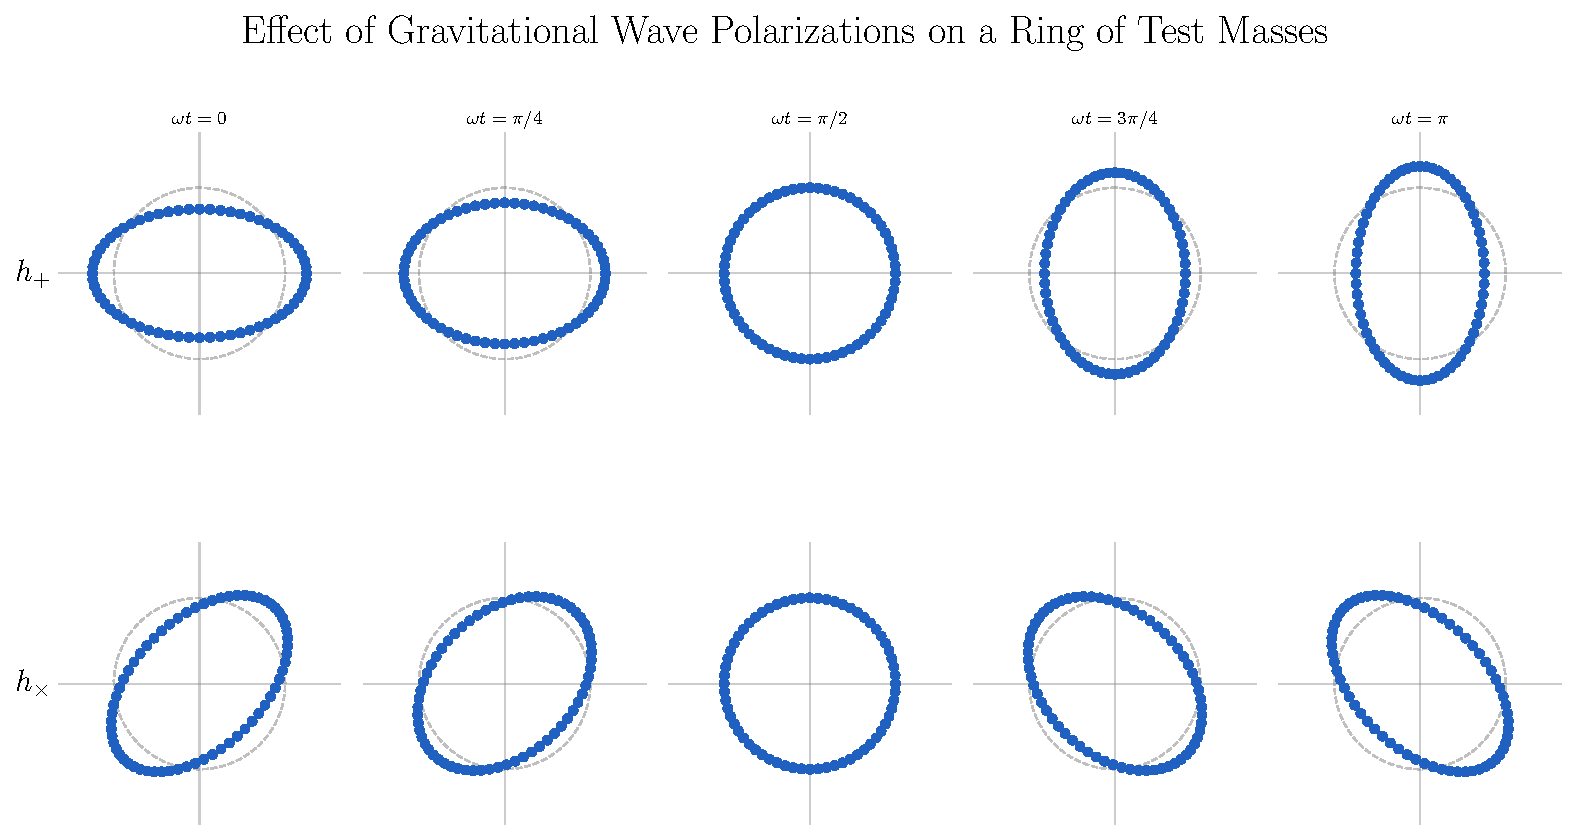
\includegraphics[width=\textwidth]{figures/test_masses.pdf}
    \caption[Effect of gravitational wave polarizations on test masses]{The effect of the two gravitational wave polarizations, $h_+$ (plus) and $h_\times$ (cross), on a ring of freely falling test masses over the course of one half period. The $h_+$ polarization stretches and compresses the ring along the $x$- and $y$-axes in turn, while the $h_\times$ polarization does the same along axes rotated by 45$^\circ$.}
    \label{intro_fig:test_masses}
\end{figure}

\section{Sources of Gravitational Waves}
\label{intro_sec:gr-source}

If we make the approximation that our source of GWs is far away and non-relativistic, it can be shown~\cite{MTW1973} that the metric perturbation in the transverse-traceless gauge is given by:
\begin{equation}
    \label{eq:quad}
    h_{ij} = \frac{2G}{c^4 r} \ddot{I}_{ij}(t - r/c)
\end{equation}
where $r$ is the distance to the source and $I_{ij}$ is the quadrupole moment tensor of the source energy density:
\begin{equation}
    I_{ij}(t) = \int x^i x^j T^{00}(t, \vec{x}) d^3x
\end{equation}
with $T^{00}$ the energy density component of the stress-energy tensor.
The prefactor $2G/c^4 \approx 10^{-44}\ \mathrm{N}^{-1}$ suppresses all but the most energetic sources beneath the level of what is observable with current technology; the most promising sources will have high energy densities and large accelerations.
In this section, I will discuss some of the sources of GWs that are targeted by the detectors discussed in Sec.~\ref{intro_sec:detectors}.

\subsection{Compact binary systems}

The most promising sources of gravitational waves for ground-based detectors are compact binary systems: pairs of black holes or neutron stars whose orbit decays due to the emission of gravitational radiation.
As a binary system loses energy to GWs, the orbital radius shrinks and the orbital frequency increases until the two bodies eventually merge.
During the inspiral, this produces a characteristic ``chirp'' signal, a sinusoidal waveform that sweeps upward in both frequency and amplitude.
The signal then transitions through a brief merger phase and a ringdown, during which the remnant -- typically a black hole, though potentially a neutron star -- radiates as it settles into its final state.

The amplitude and frequency evolution of the inspiral are determined primarily by the chirp mass
\begin{equation}
    \mathcal{M} = \frac{(m_1 m_2)^{3/5}}{(m_1 + m_2)^{1/5}},
\end{equation}
where $m_1$ and $m_2$ are the masses of the component objects.
Because the chirp mass controls the rate of frequency evolution, it is the most precisely measurable parameter from the inspiral waveform for most systems~\cite{BlEA2002}.
It also is the primary determinant of the signal amplitude, and thus the maximum distance at which a source is detectable.
In the leading post-Newtonian approximation~\cite{2014LRR....17....2B}, the characteristic strain from a CBC at luminosity distance $r$ is
\begin{equation}
    h \sim \frac{G\mathcal{M}}{c^2 r} \left(\frac{G\mathcal{M} \pi f}{c^3}\right)^{2/3},
\end{equation}
where $f$ is the instantaneous GW frequency.
The amplitude scales as $\mathcal{M}^{5/3}$; heavier systems therefore produce stronger signals and are detectable at greater distances.
This is why BBH mergers dominate the observed catalog despite their relatively low predicted astrophysical merger rates compared to BNS systems.

The coalescence of a compact binary progresses through three distinct phases.
During the \emph{inspiral}, the two bodies spiral inward as they lose energy to gravitational radiation.
The frequency evolution during this phase is well described by the post-Newtonian (PN) approximation.
For a 30+30\,$M_\odot$ BBH system, the inspiral sweeps from $\sim 10$\,Hz to several hundred hertz in a matter of seconds; for a 1.4+1.4\,$M_\odot$ BNS system, the same frequency range takes $\sim 100$\,s to traverse, posing distinct challenges for detection algorithms.
The inspiral is followed by the \emph{merger}, a brief and strongly nonlinear phase in which the two bodies collide and the GW amplitude reaches its peak.
This phase requires numerical relativity simulations to model accurately~\cite{Pretorius_2005}.
The final phase is the \emph{ringdown}, during which the remnant relaxes to its final state by emitting GWs at its characteristic quasinormal mode (QNM) frequencies~\cite{PhysRevX.9.041060}.

The first directly detected GW signal, GW150914, was produced by the merger of two black holes with total mass approximately $65\,M_\odot$~\cite{AbEA2016a}.
Note that gravitational wave events are conventionally named based on the date of their detection, so GW150914 was detected on September 14, 2015.
Since that time, the LVK has reported hundreds of CBC detections, with total masses ranging from $\sim 3\,M_\odot$ to $\sim 150\,M_\odot$~\cite{LIGOScientific:2025slb}.
Of particular scientific interest is GW170817, the first detected BNS merger, which was observed simultaneously in GWs and across the electromagnetic spectrum~\cite{AbEA2017b}.
This multi-messenger event enabled measurements of the Hubble constant~\cite{LIGOScientific:2017adf}, constraints on the neutron star equation of state~\cite{Abbott_2018}, and the identification of a kilonova~\cite{Smartt2017}.
The scientific richness of such events and the rarity of BNS mergers in the current detector network are the primary motivations for the low-latency search and parameter estimation methods developed in this dissertation.

\begin{figure}
    \centering
    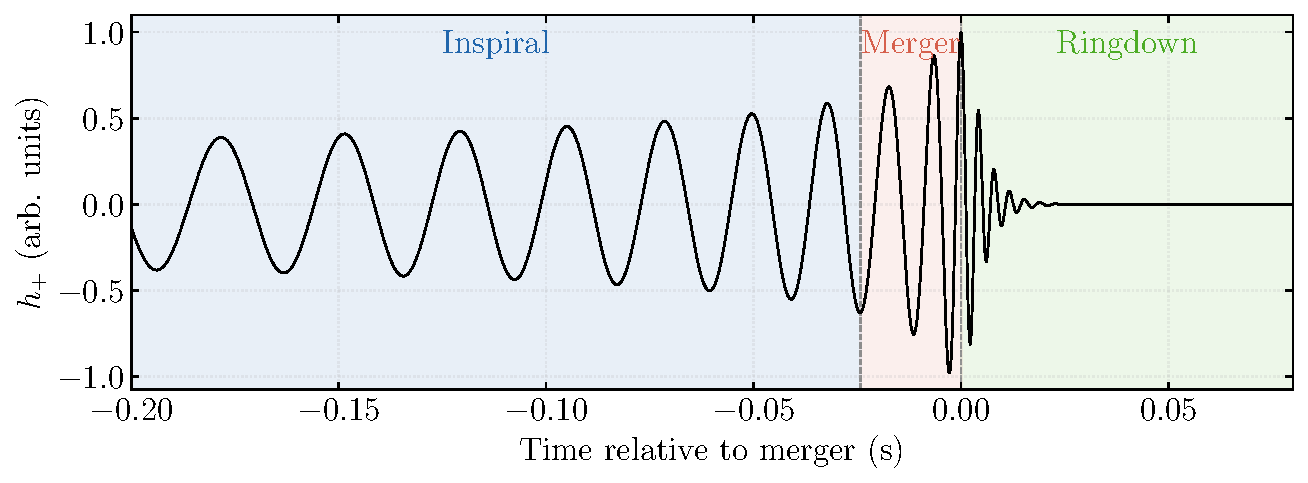
\includegraphics[width=\textwidth]{figures/cbc_phases.pdf}
    \caption[Schematic of a compact binary coalescence waveform]{Schematic of a compact binary coalescence gravitational waveform, illustrating the three phases: inspiral (chirp governed by the post-Newtonian approximation), merger (requiring numerical relativity), and ringdown (exponentially damped oscillation).}
    \label{intro_fig:cbc_phases}
\end{figure}

\subsection{Burst sources}

Gravitational wave bursts are short-duration signals whose waveform morphology cannot be predicted with sufficient accuracy to enable matched filtering (see Sec.~\ref{intro_sec:matched_filter}).
The most energetically-promising astrophysical sources are core-collapse supernovae (CCSNe), in which the asymmetric collapse of a stellar core can generate a brief burst of gravitational radiation lasting $\mathcal{O}(1)$\,s with a complex, poorly-modeled time-frequency structure~\cite{Ott_2009}.
The nonlinear, three-dimensional hydrodynamics of stellar collapse make waveform prediction impractical, so matched filtering is not a viable option.
Even with the most optimistic emission models, a galactic CCSN at $\sim 10$\,kpc would produce a strain $h \sim 10^{-21}$--$10^{-22}$ in the LIGO band, near the edge of detectability; extragalactic events are unlikely to be detectable with current instruments~\cite{Ott_2009}.
Other candidate burst sources include magnetar giant flares, accretion disk instabilities, and cosmic string cusps~\cite{Abbott_2017_burst}, all of which present similar challenges in waveform prediction.
Because of this, burst-search algorithms such as coherent WaveBurst (cWB~\cite{PhysRevD.93.042004}) look for excess power in the time-frequency domain that is coincident and coherent across multiple detectors, while remaining inconsistent with known noise transient morphologies.

\subsection{Rapidly rotating neutron stars}

A neutron star that is asymmetric about its axis of rotation will emit continuous, nearly-monochromatic gravitational waves at twice its spin frequency.
The GW strain amplitude is
\begin{equation}
    h = \frac{16\pi^2 G}{c^4} \frac{I_{zz} \epsilon f_{\rm rot}^2}{d},
\end{equation}
where $I_{zz}$ is the principal moment of inertia, $\epsilon = (I_{xx} - I_{yy})/I_{zz}$ is the equatorial ellipticity, $f_{\rm rot}$ is the rotational frequency of the neutron star, and $d$ is the distance to the source~\cite{2009ASSL..357.....B}.
Continuous wave signals are individually far below the noise floor of any single detector, so detection requires coherently integrating data over months to years to accumulate signal power.
This long integration time makes searches computationally intensive, particularly for all-sky surveys where the spin frequency, spin-down rate, and sky position are all unknown~\cite{Brady_1998}.
Targeted searches for known pulsars~\cite{Abbott_2017_continuous}, directed searches toward promising sky locations (e.g., the galactic center or the remnant of SN\,1987A)~\cite{PhysRevLett.118.121102}, and hierarchical all-sky methods~\cite{EinsteinAtHome_2009} trade sensitivity for computational efficiency.
To date, no detection of a continuous gravitational wave signal has been reported.

\subsection{Stochastic background}

The stochastic gravitational wave background (SGWB) is the superposition of a large number of individually unresolvable GW sources throughout the universe.
It is characterized by its dimensionless energy density spectrum
\begin{equation}
    \Omega_{\rm GW}(f) = \frac{f}{\rho_c} \frac{d\rho_{\rm GW}}{df},
\end{equation}
where $\rho_{\rm GW}$ is the gravitational wave energy density, $\rho_c = 3H_0^2 / (8\pi G)$ is the critical energy density of the universe, and $H_0$ is the Hubble constant.
The SGWB is expected to be an approximately stationary, Gaussian noise-like signal.
Therefore, in any single detector, it is indistinguishable from instrumental noise.
Searches for the SGWB instead use the cross-correlation between detectors: a common GW background produces correlated strain in each detector whose magnitude is described by the overlap reduction function $\gamma(f)$.
The optimal cross-correlation estimator integrates this signal over long observation times, with sensitivity improving as $T^{1/2}$~\cite{AlRo1999}.
Recent observations by pulsar timing arrays (PTAs) have reported evidence for a SGWB at nHz frequencies, consistent with the expected Hellings-Downs spatial correlation pattern~\cite{NANOGrav_2023}, marking the first indirect detection of a stochastic gravitational wave signal.
In the sensitive band of the LIGO detectors, the astrophysical CBC background is predicted to be near or below current sensitivity, and no detection has been reported~\cite{o4_stochastic}.

\section{LIGO Detectors}
\label{intro_sec:detectors}

LIGO consists of two large-scale interferometric detectors located in Hanford, Washington and Livingston, Louisiana~\cite{Aasi_2015}.
Each detector is a Michelson interferometer with 4\,km-long arms that measure the differential change in length caused by passing gravitational waves.
When a GW with amplitude $h$ passes through the detector, it produces a differential strain $\Delta L/L = h/2$ in each arm, where $L = 4$\,km.
The detectors are designed to measure strains as small as $h \sim 10^{-23}\,\mathrm{Hz}^{-1/2}$ near their most sensitive frequencies, corresponding to a change in arm length of $\sim 10^{-20}\,\mathrm{m}$, many orders of magnitude smaller than the diameter of a proton.

Several enhancements to the basic Michelson design are used to achieve this sensitivity; here I describe a few of the most significant features, though there are many more that are not discussed here.
The arm cavities contain Fabry-Perot resonators, in which light bounces between two highly reflective mirrors many hundreds of times before exiting.
This increases the effective path length of the interferometer, allowing the GW-induced phase shift to accumulate over a longer distance and thus increase the detector's sensitivity to GWs.
Because the detectors operate near a dark fringe, almost all light is reflected toward the laser.
A power recycling mirror, placed between the laser and the beam splitter, reflects this light back into the beam arms, increasing the circulating power in the arms by a factor of $\sim 40$~\cite{Izumi_2017} and reducing shot noise.
Similar to the power recycling mirror, a signal recycling mirror is placed between the beam splitter and the photodetector at the output port of the interferometer.
This mirror forms a resonant cavity with the arm cavities, and tuning the size of this cavity allows the detector's frequency response to be modified.
In practice, the signal recycling cavity is tuned to broaden the detector's bandwidth, improving sensitivity at high frequencies at the cost of some sensitivity at low frequencies~\cite{Aasi_2015}.
These features are shown in Fig.~\ref{intro_fig:ligo_layout}.

\begin{figure}[t]
    \centering
    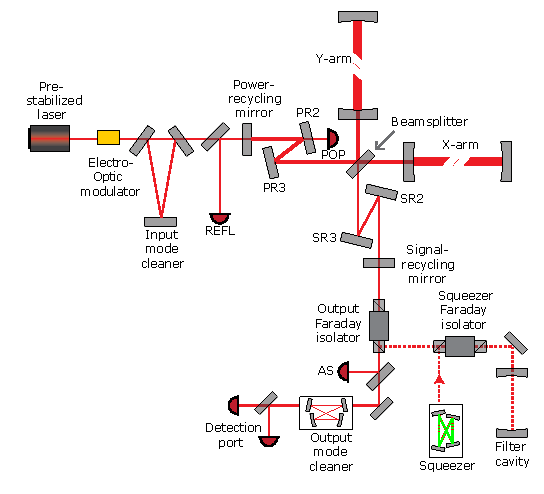
\includegraphics[width=0.8\textwidth]{figures/ligo_layout.pdf}
    \caption[Optical layout of the Advanced LIGO interferometer]
    {
        Schematic of the Advanced LIGO interferometer, showing the Fabry-Perot arm cavities, power recycling mirror (PRM), signal recycling mirror (SRM), and the main optical path from laser to photodetector.
        Reproduced from Fig.~1 of Ref.~\cite{o4_performance}.
    }
    \label{intro_fig:ligo_layout}
\end{figure}

The sensitivity of the LIGO detectors is limited by different noise sources in different frequency bands~\cite{o4_performance}.
At low frequencies ($\lesssim 50$\,Hz), the dominant noise source controls noise from suspension damping, though the Livingston detector noise also has a significant contribution from seimic activity in this frequency range.
At intermediate frequencies (roughly 50--500\,Hz), the noise is dominated by a combination of thermal fluctuations in the mirror coatings and quantum shot noise, the statistical uncertainty in the number of photons detected at the output photodetector.
At high frequencies ($\gtrsim 500$\,Hz), the sensitivity is limited almost entirely by quantum shot noise.
The amplitude spectral density of the LIGO detectors during O4a, along with the Advanced LIGO design sensitivity, is shown in Fig.~\ref{intro_fig:asd_comparison}.

\begin{figure}
    \centering
    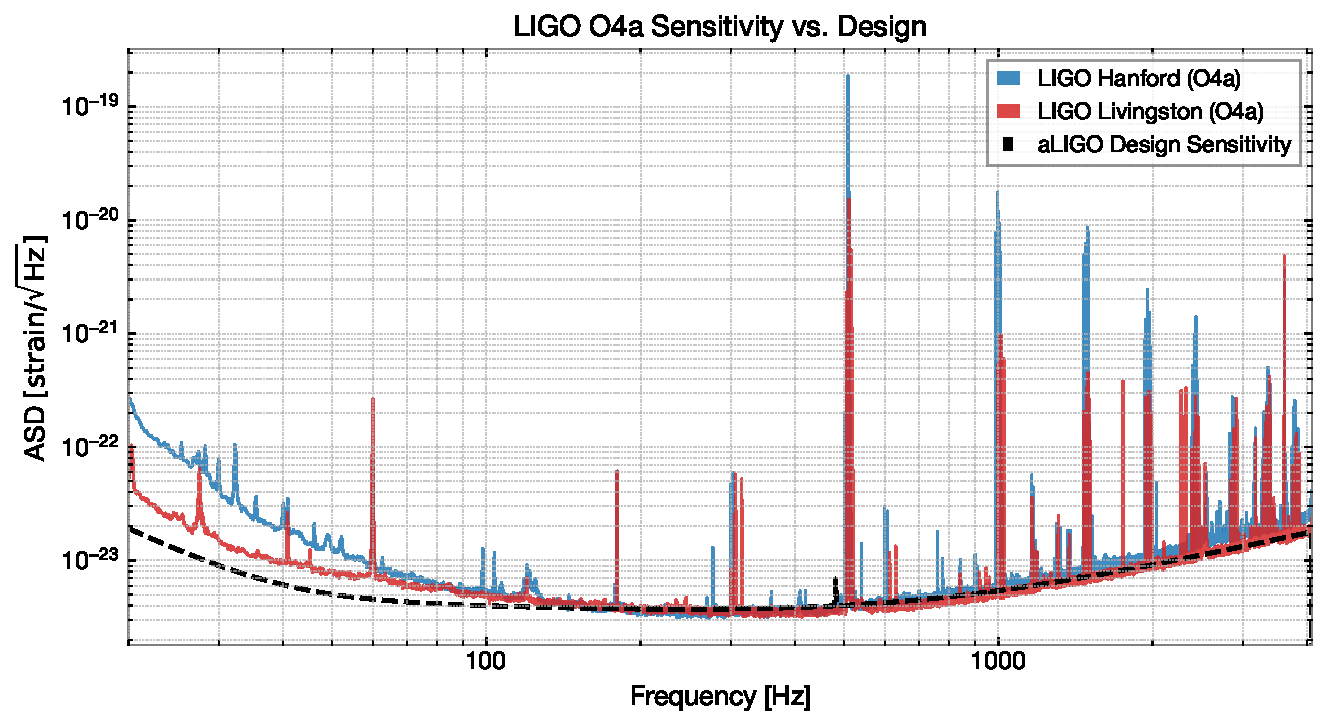
\includegraphics[width=\textwidth]{figures/asd_comparison.pdf}
    \caption[Amplitude spectral density of the LIGO Hanford and Livingston detectors during O4a]{Amplitude spectral density of the LIGO Hanford (H1) and Livingston (L1) detectors estimated from a 2048-second segment during the fourth observing run (O4a), compared to the Advanced LIGO design sensitivity. 
    The most significant peaks come from the violin modes of the fused silica suspension fibers, with the fundamental frequency just below 500\,Hz and harmonics at integer multiples~\cite{Aston_2012}.}
    \label{intro_fig:asd_comparison}
\end{figure}

Beginning with O4, Advanced LIGO employs frequency-dependent squeezed light injection to further reduce quantum noise~\cite{Tse_2019}.
Squeezed states of light reduce the quantum uncertainty in the phase quadrature below the vacuum level, lowering shot noise at high frequencies.
Frequency-dependent squeezing, achieved by rotating the squeezing ellipse as a function of frequency using an external filter cavity, allows simultaneous reduction of shot noise at high frequencies and quantum radiation pressure noise at low frequencies.
This technique has contributed measurably improved sensitivity across the detector band in O4 relative to O3.

Operating multiple detectors simultaneously is essential for gravitational wave astronomy.
A network of geographically separated detectors can localize a source through triangulation based on the differences in arrival time between detectors, with each additional detector providing more information for localization.
The LIGO detectors have been joined by the Advanced Virgo detector in Cascina, Italy~\cite{Acernese_2015}, and the KAGRA detector in Kamioka, Japan~\cite{kagra}, forming a multi-detector network.
Unlike optical telescopes, these ground-based detectors are broadly omnidirectional, but individual detectors have blind spots where the antenna response vanishes.
Non-co-located, non-co-aligned detectors in a network fill in these blind spots and ensure that sources near any single detector's null direction can still be detected and localized by the full network.
Sky localization with this network enables electromagnetic follow-up observations of GW events, one of the primary scientific motivations for the low-latency methods developed in this dissertation.

\section{Matched Filtering}
\label{intro_sec:matched_filter}

The traditional approach to detecting gravitational wave signals in LIGO data is matched filtering~\cite{CuFl1994}.
Given a data stream $d(t) = n(t) + h(t)$, where $n(t)$ is detector noise and $h(t)$ is a GW signal, the matched filter is the linear filter that maximizes the signal-to-noise ratio (SNR) when the form of $h(t)$ is known.
For stationary Gaussian noise with one-sided power spectral density (PSD) $S_n(f)$, the optimal filter is the template waveform itself, weighted by the inverse of the noise PSD.
The resulting SNR time series is
\begin{equation}
    \rho^2(t) = 4 \Re \int_0^\infty \frac{\tilde{d}(f)\, \tilde{h}^*(f)}{S_n(f)}\, e^{2\pi i f t}\, \mathrm{d}f,
\end{equation}
where tildes denote Fourier transforms.
A peak in $\rho(t)$ above a detection threshold indicates the presence of a signal whose waveform matches the template, and the time of the peak estimates the coalescence time.

Because the parameters of a gravitational wave signal are not known in advance, matched filtering searches use a template bank containing a large number of templates with different parameters~\cite{Owe1996}.
Templates are placed in parameter space such that no signal of interest falls more than some maximum distance away from the nearest template.
Hundreds of thousands to millions of templates may be required to cover the full parameter space of interest, making the computational cost of matched filtering searches substantial.
The number of templates required to cover a given parameter space scales steeply with the minimum component mass: lighter systems have longer, more rapidly evolving waveforms that require finer sampling in chirp mass to keep the signal mismatch below the desired threshold.
An illustration of the matched filtering process is shown in Fig.~\ref{intro_fig:matched_filter}.

\begin{figure}[t]
    \centering
    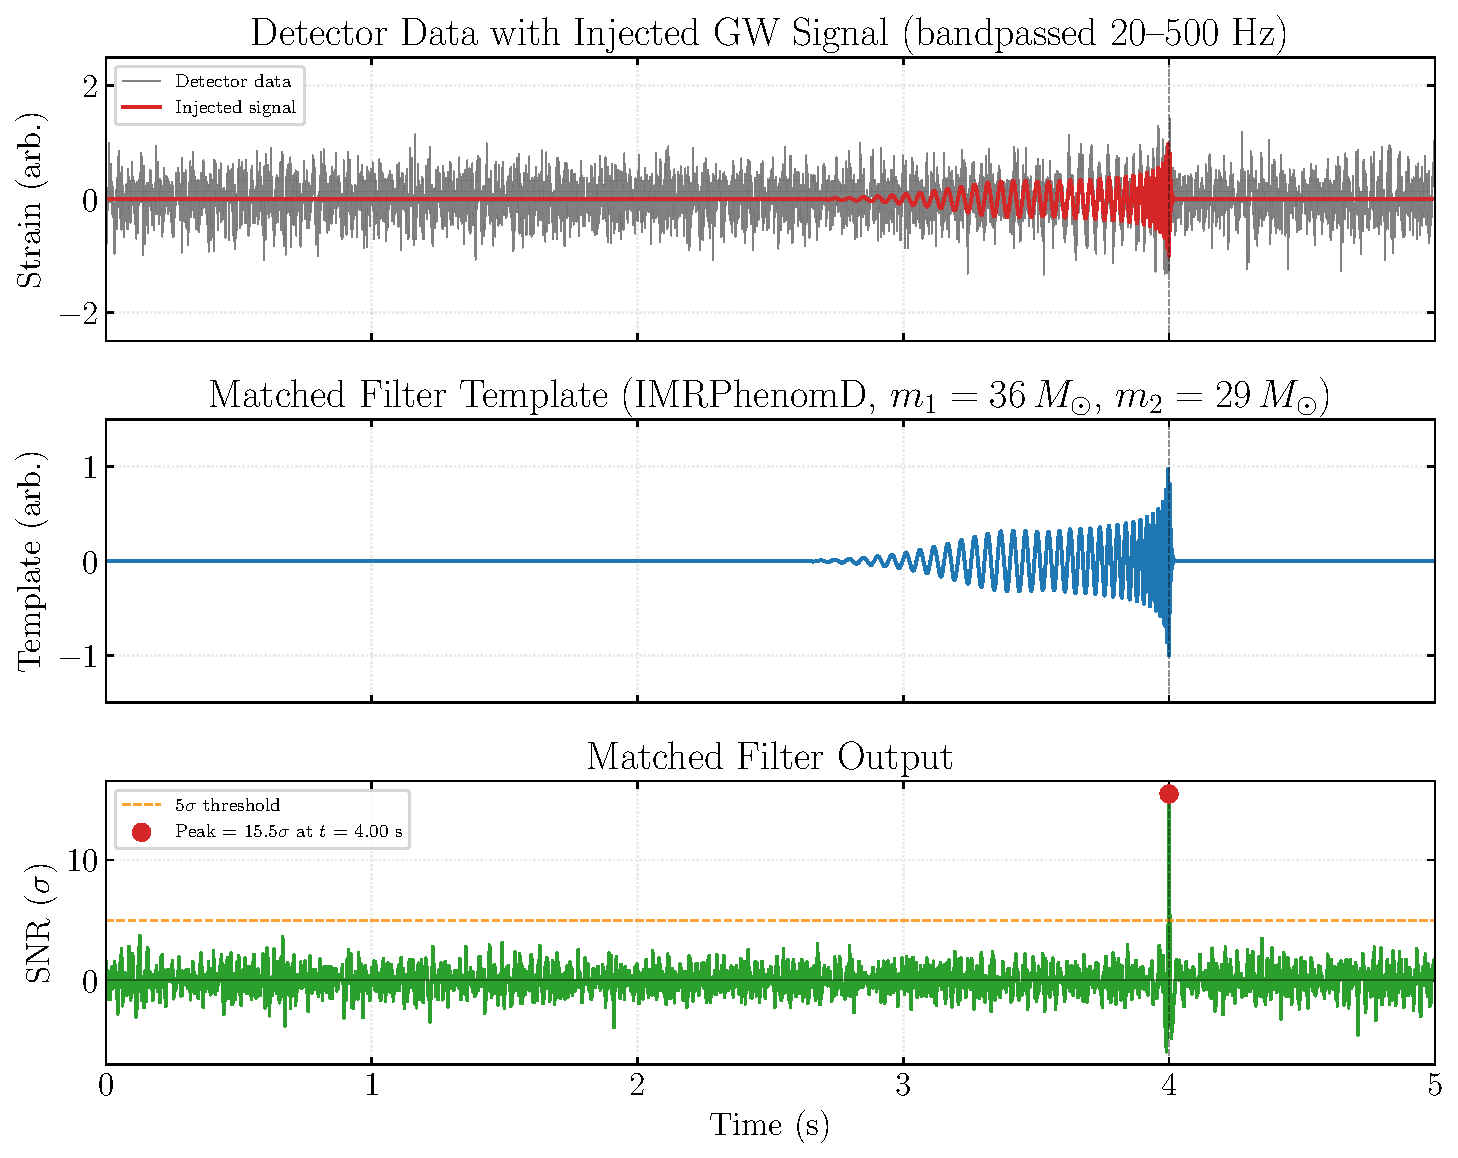
\includegraphics[width=0.95\textwidth]{figures/matched_filter.pdf}
    \caption[Illustration of the matched filtering technique]{Illustration of matched filtering applied to a simulated gravitational wave signal. \textit{Top}: bandpassed detector data containing an injected CBC signal (red). \textit{Middle}: the matched filter template (CBC waveform). \textit{Bottom}: the matched filter output SNR time series, normalized by its standard deviation far from the signal, showing a peak at the true merger time.}
    \label{intro_fig:matched_filter}
\end{figure}

The time-frequency morphology of a CBC signal is an upward-sweeping track (shown in the Q-transform spectrogram of Fig.~\ref{intro_fig:qtransform}) that is qualitatively distinct from typical noise transients in detector data, known as ``glitches''.
Despite this distinction, glitches can still produce a large matched filter SNR and mimic a true signal, making signal-based vetoes necessary for rejecting false triggers.
A commonly-used method is the $\chi^2$ time-frequency veto~\cite{Allen_2005}, which divides the matched filter output into sub-bands and tests whether the SNR accumulated in each is consistent with what a true GW signal would produce.
A glitch that, for example, concentrates power in a narrow frequency band will fail this test and receive a reduced ranking statistic.

\begin{figure}
    \centering
    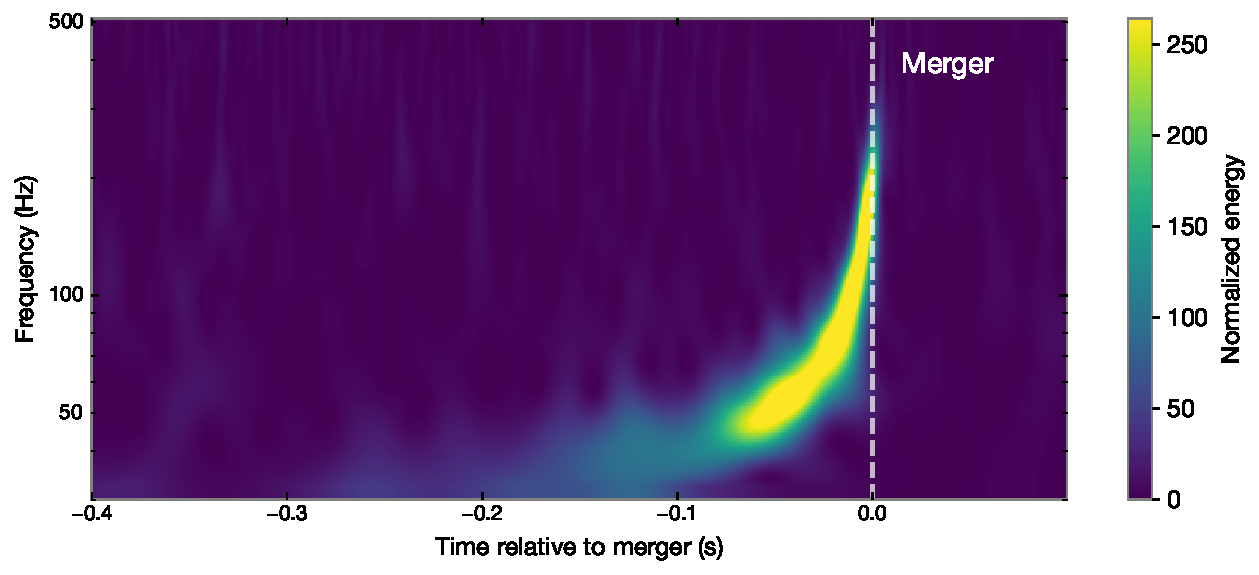
\includegraphics[width=\textwidth]{figures/qtransform.pdf}
    \caption[Q-transform spectrogram of a simulated binary black hole signal]{Q-transform spectrogram of a simulated GW150914-like binary black hole signal ($m_1 = 36\,M_\odot$, $m_2 = 29\,M_\odot$) embedded in aLIGO-design colored noise. 
    The characteristic chirp track is visible as a bright upward-sweeping curve, with the gravitational-wave frequency rising from $\sim$30\,Hz roughly 0.25 seconds before merger (dashed white line) to $\sim$200\,Hz at coalescence. 
    This morphology is qualitatively distinct from that of detector glitches, and is the basis for the signal-consistency tests used to distinguish astrophysical signals from noise transients.}
    \label{intro_fig:qtransform}
\end{figure}

The matched-filter searches used by the LVK (GstLAL~\cite{Tsukada_2023}, MBTA~\cite{Allene_2025}, PyCBC~\cite{Dal_Canton_2021}, and SPIIR~\cite{PhysRevD.105.024023}) operate in low latency, producing triggers for real-time alerts to the astronomical community.
The machine learning search developed in this dissertation is complementary to matched filtering: it operates at much lower computational cost and lower latency, and implicitly learns to distinguish signals from glitches through training on realistic data, rather than applying analytical signal-consistency tests.

\section{Bayesian Parameter Estimation}
\label{intro_sec:bayesian_pe}

Once a GW signal has been identified by a search pipeline, the goal of parameter estimation (PE) is to infer the posterior probability distribution of the parameters of the source, $\boldsymbol{\theta}$, given the observed data $d$.
These parameters include the component masses, spins, sky location, distance, and inclination of the binary merger.
This is accomplished via Bayes' theorem:
\begin{equation}
    p(\boldsymbol{\theta} \mid d) = \frac{\mathcal{L}(d \mid \boldsymbol{\theta})\, \pi(\boldsymbol{\theta})}{p(d)},
\end{equation}
where $\mathcal{L}(d \mid \boldsymbol{\theta})$ is the likelihood of the data given a signal with parameters $\boldsymbol{\theta}$, $\pi(\boldsymbol{\theta})$ is the prior distribution encoding knowledge and assumptions about the source population, and $p(d) = \int \mathcal{L}(d \mid \boldsymbol{\theta})\, \pi(\boldsymbol{\theta})\, d\boldsymbol{\theta}$ is the evidence, which normalizes the posterior.

\begin{figure}[t]
    \centering
    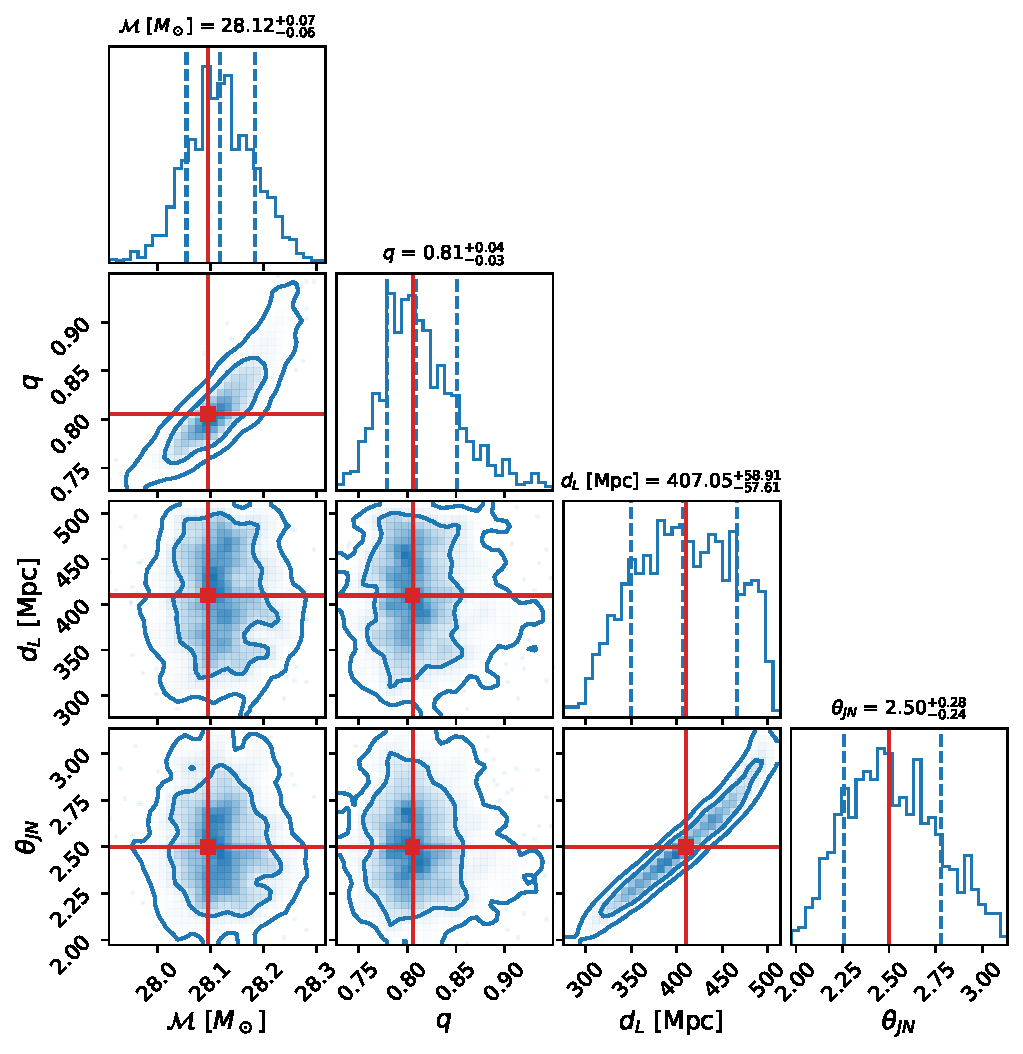
\includegraphics[width=0.65\textwidth]{figures/pe_corner.pdf}
    \caption[Bayesian parameter estimation posteriors for a simulated binary black hole signal]{Corner plot of the marginalized posterior distributions for a simulated GW150914-like binary black hole signal ($m_1 = 36\,M_\odot$, $m_2 = 29\,M_\odot$, $d_L = 410\,\mathrm{Mpc}$), inferred using the Bilby PE framework with an IMRPhenomD likelihood and the dynesty nested sampler. 
    The diagonal panels show 1D marginal posteriors with 68\% credible intervals marked; the off-diagonal panels show 2D marginals at the 68\% and 95\% credible levels. 
    Red lines indicate the injected parameter values. 
    }
    \label{intro_fig:pe_corner}
\end{figure}

Assuming a network of detectors with stationary Gaussian noise, the log-likelihood takes the form
\begin{equation}
    \ln \mathcal{L}(d \mid \boldsymbol{\theta}) = -\frac{1}{2} \sum_k \langle d_k - h_k(\boldsymbol{\theta}) \mid d_k - h_k(\boldsymbol{\theta}) \rangle,
\end{equation}
where the sum runs over detectors, $h_k(\boldsymbol{\theta})$ is the waveform template projected onto detector $k$, and $\langle a \mid b \rangle = 4\, \Re \int_0^\infty \tilde{a}(f)\tilde{b}^*(f) / S_n(f)\, df$ is the noise-weighted inner product from Sec.~\ref{intro_sec:matched_filter}.
Evaluating this likelihood requires computing a waveform template $h_k(\boldsymbol{\theta})$ at each point in parameter space.
Standard approaches use stochastic sampling algorithms, such as Markov chain Monte Carlo (MCMC) or nested sampling~\cite{Skilling_2006}, to draw samples from the posterior without evaluating the full integral.
The LVK PE codes LALInference~\cite{lalinference_paper} and Bilby~\cite{Ashton_2019} implement these samplers, typically requiring $\mathcal{O}(10^7)$ likelihood evaluations and times of hours to days per event.
An example of the resulting posterior is shown in Fig.~\ref{intro_fig:pe_corner}: the chirp mass is constrained to a fraction of a solar mass, while the mass ratio, luminosity distance, and inclination each carry substantially larger fractional uncertainties.
This computational cost is the primary obstacle to rapid source characterization following a GW detection, and motivates the machine learning approach presented in this dissertation.

\section{Machine Learning for Gravitational-Wave Astronomy}
\label{intro_sec:ml}

The traditional approaches described above -- matched filtering and Bayesian parameter estimation -- are well-founded and highly effective, but each faces practical limitations.
Matched filtering is optimal when the signal model is known exactly and the noise is stationary and Gaussian; in practice, neither condition holds perfectly, as real detector noise shifts over time and contains non-Gaussian glitches.
Bayesian PE, while statistically rigorous, is computationally expensive and too slow for full parameter estimation in real-time.
Machine learning (ML) offers a complementary approach that addresses both limitations: it learns properties of signal-like and noise-like data from labeled examples rather than requiring an explicit signal model, and amortizes the cost of inference over a training phase so that individual events can be analyzed in seconds.

A neural network classifier trained on realistic detector data, both with and without simulated signals, learns an internal representation of the data that can be used to predict whether a signal is present~\cite{PhysRevLett.120.141103}.
This implicit encoding of signal morphology replaces the explicit template bank required by matched filtering.
Gravitational-wave data analysis is particularly well-suited for ML: multiple geographically separated detectors allow effectively unlimited samples of background noise by time-shifting the data streams relative to one another, and high-fidelity waveform models derived from GR allow as many simulated signals as desired.

For parameter estimation, a class of ML models called \emph{normalizing flows} provides a natural framework.
A normalizing flow is a learned, invertible mapping between a simple base distribution and a complex target distribution~\cite{papamakarios2021normalizing}, where here the target distribution is the posterior probability of source parameters given observed data.
Once trained on simulated events, the flow can evaluate the posterior probability at the cost of a single forward pass through the network rather than the millions of likelihood evaluations required by traditional Markov chain Monte Carlo or nested sampling methods.
This enables posterior estimation in under two seconds, compared to hours or days for full Bayesian samplers.

The detection and parameter estimation algorithms developed in this dissertation are based on these properties, achieving performance competitive with traditional methods while operating at significantly lower computational cost and latency.

%%%%%%%%%%%%%%%%%%%%%%%%%%%%%%%%%%%%%%%%%%%%%%%%%%%%%%%%%%%%%%%%%%%%%%%%%%%%%%%%

\singlespacing
\begingroup
\emergencystretch=3em
\printbibliography[title=References,heading=subbibintoc]
\endgroup
\end{refsection}